%!TEX root = ../template.tex
%%%%%%%%%%%%%%%%%%%%%%%%%%%%%%%%%%%%%%%%%%%%%%%%%%%%%%%%%%%%%%%%%%%%
%% chapter3.tex
%% NOVA thesis document file
%%
%% Chapter with a short latex tutorial and examples
%%%%%%%%%%%%%%%%%%%%%%%%%%%%%%%%%%%%%%%%%%%%%%%%%%%%%%%%%%%%%%%%%%%%

\typeout{NT FILE chapter3.tex}%

\makeatletter
\newcommand{\ntifpkgloaded}{%
  \@ifpackageloaded%
}
\makeatother


\chapter{Elaboration}\label{cha:elaboration}

In this chapter, we give a conceptual overview of the proposed solution. We begin by presenting the general overview of the system model and the design goals in Section~\ref{sec:system_model}, followed by a more technical description of the techniques and technologies used in the implementation of the prototype in Section~\ref{sec:prototype_guidelines}. Finally, we present how we intend to test and validate our implementation in Section~\ref{sec:validation}.

\section{System Model}\label{sec:system_model}

In this section, we present the system model of our proposed solution. We start by presenting the foundation of our work in Section~\ref{subsec:initial_system_model_approach}, where we explore the current Tor Relay internal architecture and how we intend to extend its architecture. In Section~\ref{subsec:our_system_model_approach}, we present our approach to enhance the privacy of Tor users by integrating a Differential Privacy mechanisms in Tor relays and on the Client side. Finally, in Section~\ref{subsec:differential_privacy_approach}, we present the \textit{Differential Privacy Scheduler}, or \textit{DP Scheduler}, which is a component that maintains the circuit queues and is responsible for selecting the cells to be allocated in the output buffer, just like the vanilla Tor scheduler.

\subsection{Initial System Model Approach}\label{subsec:initial_system_model_approach}

As shown in Section~\ref{sec:problem}, Tor is a widely used network for anonymous communication. However, it has been proven that some vulnerabilities that can be exploited by attackers to de-anonymize users, such as traffic analysis attacks. Several techniques have been proposed to mitigate these attacks, such as \(k\)-Anonymity, but they lack formal guarantees of privacy and are almost based on practical validations, which in real-world applications might vary. In this context, we propose a new approach to enhance the privacy of Tor users by integrating a Differential Privacy mechanisms in Tor relays and on the Client side. Our approach aims to develop a Differential Private Scheduler similar to KIST (Section~\ref{subsubsec:kist}) and a Client Side Proxy that will be responsible for adding noise to the traffic flows in order to keep users anonymous. 
The Tor scheduler handles two buffers, input and output. The first receives the cells and the second sends them. Between these two buffers, the circuit queue is responsible for managing the cells that are being processed. 

\begin{figure}
    \centering
    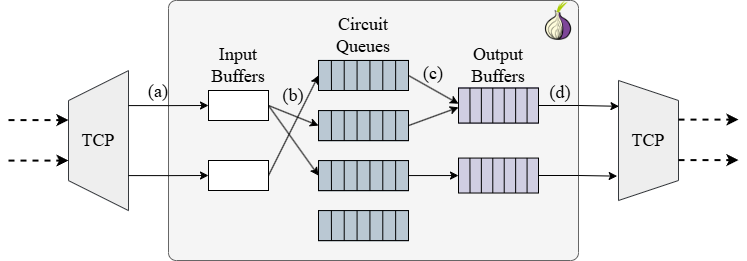
\includegraphics[width=0.8\textwidth]{Chapters/Figures/Fig1.png}
    \caption{Tor Relay Internal Architecture}\label{fig:initial_system_model}
\end{figure}

The Tor Relay Internal Architecture is shown in Figure~\ref{fig:initial_system_model}. 
When a relay receives a TCP packet, the kernel processes them and delivers to Tor (Figure~\ref{fig:initial_system_model} (a)).
Upon receiving the entire packet, Tor onion-encrypts it and the cell is enqueued into the circuit queue (Figure~\ref{fig:initial_system_model} (b)). 
Each circuit queue represents a circuit that the relay maintains. In this example, this relay is part of 4 circuits, each with a different circuit queue. Nonetheless, this does not mean that the relay must have an input buffer for each circuit, since a single TCP connection may be part of multiple circuits. 
The scheduler is responsible for selecting a cell from the circuit queue to be sent to the output buffer (Figure~\ref{fig:initial_system_model} (c)).
Finally, when the relay's output buffer contains sufficient data to form a TLS packet, the data is sent via TCP connection (Figure~\ref{fig:initial_system_model} (d))~\cite{KIST, EWMA}.

\subsection{Our System Model Approach}\label{subsec:our_system_model_approach}

The Tor Relay described in Figure~\ref{fig:initial_system_model} represents a simple relay. Our goal is to provide formal guarantees of privacy to users of Tor Network whilst maintaining practical levels of performance. To achieve this goal, we propose a new approach to enhance the privacy of Tor users by integrating a Differential Privacy mechanisms in Tor relays and on the Client side. 
Our approach aims to develop a differential private mechanism, called \textit{Differential Privacy Scheduler Component}, that is responsible for adding noise to the traffic flows based on several parameters in order to protect the privacy of users.  
\begin{figure}[!h]
    \centering
    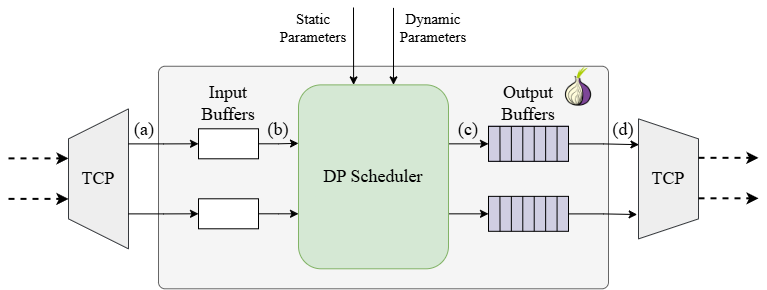
\includegraphics[width=0.8\textwidth]{Chapters/Figures/Fig2_dp.png}
    \caption{Enhanced Tor Relay with Differential Privacy Scheduler Component}\label{fig:our_system_model}
\end{figure}
Figure~\ref{fig:our_system_model} illustrates the enhanced Tor Relay internal architecture with our \textit{Differential Privacy Scheduler Component}. 
In addition, to streghen anonymity between the client and the Bridge or Entry Node, we also intend to develop a Client Side Proxy that will contain a similar Differential Privacy Scheduler. The scheduler must be added to the Client Side to obfuscate the traffic in the weaker part of the Tor communication, which is the first hop between the client and the Bridge or Entry Node. We believe that Pluggable Transports, as refered in Section~\ref{subsec:tor_bridges}, can be used together with our solution to provide a better privacy to users.
These components are responsible for adding noise and control to the traffic flow, focusing on improving the circuit queue scheduler algorithm, and variable levels of performance and privacy, according to the parameters set by the relay or dynamically calculated.   

\subsection{Differential Privacy Scheduler}\label{subsec:differential_privacy_approach}

The \textit{Differential Privacy Scheduler}, or \textit{DP Scheduler}, is a component that manages the circuit queues and is responsible for selecting the cells to be allocated in the output buffer, similar to the vanilla Tor scheduler. In addition, the \textit{DP Scheduler} uses a set of parameters to allow customization, by the relay operator and accordingly to the system conditions, on the level of privacy and performance. These parameters can be split into two categories: \textit{configuration} and \textit{dynamic}. 

This component represents a subtle change in the Tor Relay internal architecture, but we believe that it can significantly improve users' privacy, based on the Differential Privacy formal guarantees that we aim to provide.

\subsubsection{Configuration Parameters}\label{subsubsec:configuration_parameters}

Our work aims to provide a configurable file that allows the relay operator to set the \textit{Configuration}, or \textit{Static}, Parameters before deploying the relay.
One of these parameters is the queue size, called privacy window, which can have two different approaches: the \textit{privacy window length} determines the number of cells that the \textit{DP Scheduler} will consider executing the differential private algorithm and, therefore, apply noise into this window and subsequently into the traffic; the other approach, called \textit{privacy window time interval} determines the time, in milliseconds, to fill a buffer and, when the timer ends, the differential private mechanism is applied on the received packets. We will consider implementing both approaches in our prototype. 
Another static parameter is the \textit{privacy parameter}, denoted by $\epsilon$, which is the input of the Differential Privacy Mechanism, as refered in Section~\ref{sec:differential_privacy} and determines the level of privacy that the \textit{DP Scheduler} will provide. Our work aims to provide a configurable file that allows the relay operator to set these parameters before running the relay.

\subsubsection{Dynamic Parameters}
These parameters are calculated by the \textit{DP Scheduler} based on the current state of the relay and the network. An example of dynamic parameter is the allowed interval of latency that our system must aim to provide. In this case, the \textit{DP Scheduler} will calculate the noise to be added to the traffic in order to maintain the latency within the allowed interval. If the latency is above the interval, the value of the static parameters \(\epsilon\) may be lowered, reducing the noise injection and, therefore, improving the performance.


\section{Prototype Guidelines}\label{sec:prototype_guidelines}

In order to implement the proposed solution, we have 2 main approaches: the Tor~\cite{dingledine2004tor} approach and the MIRACE~\cite{MIRACE} approach. Both approaches aim to provide a solution to the vulnerability of Anonymity Networks, such as Tor, to fingerprinting and correlation attacks, by using Differential Privacy mechanisms, and to provide formal privacy guarantees whilst maintaining reasonable performance levels. To achive these goals, both approaches intend to develop an internal compenent of the networks' relay nodes that can inject noise into the traffic flows in order to protect users' anonymity. In this section, we present both approaches and how we intend to implement them.

\subsection{The Tor Approach}\label{subsec:tor_approach}

Firstly, we will consider the approach based on extending the Tor Relay Scheduler Software Architecture with the implementation of a differential private mechanism capable of adding sufficient noise to the traffic flows that is able to minimize website fingerprinting and correlation attacks effectiveness on the Tor Network, therefore protecting the privacy of users. 
To implement this approach, we will use the already existing Tor source code, more specifically the scheduler component (\texttt{scheduler.h}). This approach aims to modify the \texttt{scheduler.h} file and add our differential private scheduler as part of the \texttt{scheduler\_type\_t} enum, which already contains the vanilla and the KIST~\cite{KIST} schedulers. In addition, we aim also to develop a new scheduler, using the Tor Scheduler Interface \texttt{scheduler\_t}, which implements the necessary functions in order to fit our design into Tor system. This way, the file `scheduler\_dp.c' would be added to the Tor source code.

The source code is written in C language and, even though there has been some efforts to export the C code base~\cite{TorRepo} to Rust code base~\cite{TorRustRepo}, after analyzing both sources, we decided to only implement in the C language, considering that, at the time of our work, the Rust source code only represents a fraction of the Tor system, and we believe that it could affect the validation of our work.
This approach aims to improve Tor system by providing greater guarantees and formal proofs of privacy, and we aim to maintain reasonable performance results in order to the scheduler to be considered as an option for Tor users which may consider sacrificing some performance in order to have a better privacy. 

\subsection{The MIRACE Approach}\label{subsec:mirace_approach}

On the other hand, we also propose another approach for the implementation of our Differential Private Component, by extending the MIRACE work. This way, we believe that merging both Path Splitting techniques and Differential Privacy mechanisms can provide a better privacy. This work is based on another NOVA LINCS work called TorKameleon~\cite{TorKameleon}, which is developed in Go language. The MIRACE approach consists of implementing the \textit{Differential Privacy Scheduler Component} in each Relay Node used in the MIRACE network. Additionally, we aim to augment the scheduler with a formal and differential private mechanisms to leverage the MIRACE multi-path algorithm. We believe that combining traffic splitting and multipath multi-encapsulation techniques from MIRACE with the Differential Privacy mechanisms from our work can provide a better privacy to Tor users.
This approach is the alternative to the Tor approach, considering that Tor source code may be more complex and harder to implement in the time frame of this work. On the other hand, the MIRACE approach uses Golang which is a simpler language and both MIRACE and TorKameleon authors represent a great support to our work.

\section{Validation}\label{sec:validation}

The main goal of this work is to provide a viable solution to the current privacy issues in Anonymity Networks, such as Tor, by using Differential Privacy mechanisms to provide formal privacy guarantees whilst maintaining reasonable performance levels. Using DP algorithms, we aim to provide a solution that can decrease the efficiency of correlation attacks and website fingerprinting.

In order to validate our solution and present a trustworthy conclusion of whether our work is useful to the current Anonymity Networks State-of-the-Art or it can be ruled out for future work and reference, we will present two main types of validation: Performance Measurements and Unobservability Measurements. To execute our validation, we intend use Shadow~\cite*{Shadow, Shadow2}, which is a specific experimentation tool that allows us to test and simulate the Tor Network in a simulated environment, leading to a more controlled but easier prototype implementation and validation. Also, this tool was used by the KIST work~\cite{KIST} to validate their solution, which was eventually introduced into the Tor source. 

\subsection{Unobservability Measurements}\label{subsec:unobservability_measurements}

Unobservability is the main goal of our work. We aim to prove that Differential Privacy mechanisms can provide strong and quantifiable privacy guarantees to users of Anonymity Networks, such as Tor. To test unobservability, we will consider using state-of-the-art Machine/Deep Learning models to simulate attacks on our solutions.

To simulate the attacks, we will consider using the following works:
\paragraph{DeepCoFFEA~\cite{DeepCoFFEA}:} Motivated by DeepCorr~\cite{DeepCorr}, DeepCoFFEA is a flow correlation attack that combines deep learning to train a pair of feature-embedding networks that respectively map Tor and exit flows into a single low-dimensional space where correlated flows are similar; pairs of embedded flows can be compared at lower cost than pairs of full traces, and also uses amplification, dividing flows into short windows and using voting across these windows to significantly reduce false positives.

\paragraph{FINN~\cite{FINN}:} FINN is a flow fingerprinting technique that leverages neural networks and generates and adds slight perturbations into live flow which allows to fingerprint the traffic. This work is also based on DeepCorr~\cite{DeepCorr}.

\paragraph{TorMarker~\cite{TorMarker}:} TorMarker uses traffic time-based watermarking and deep learning of traffic time properties to de-anonymize connections made through Tor. This work is based on concepts similar to DeepCorr~\cite{DeepCorr} and FINN~\cite{FINN}.

\paragraph{TirDeanon~\cite{TirDeanon}:} Finally, TirDeanon is a traffic de-anonymization tool inspired in deep learning techniques that can establish traffic flow correlations and de-anonymize Tor users. 

\paragraph{} With this set of tools, we aim to prove that our solution can affect negatively the effectiveness of fingerprinting and correlation attacks, by using Differential Private mechanisms to add noise to the traffic flows, and also confirm the formal privacy guarantees that we intend to provide to users of Anonymity Networks, such as Tor and MIRACE.


\subsection{Performance Measurements}\label{subsec:performance_measurements}

Even though the main goal of our work focus on anonymity and the effectiveness of Differential Privacy, we consider performance to be an important element to the success of our solution, which can be the difference between a viable solution, useful in real-world applications, and a theoretical solution which works but does not provide a real-world application due to low performance.

This way, we aim to provide an extensive and detailed analysis of the performance of our solution. In order to achieve this, we will consider metrics, such as latency, throughput and resources allocation, and some different scenarios where we can stress our solution in different ways, leading to a more detailed and broad analysis of the performance of our solution. We will have 5 main scenarios:
\paragraph{iPerf:} This tool will be used to measure some critical metrics, such as latency and throughput, but also the jitter and packet loss that our solution may introduce.

\paragraph{Web Browsing:} In this scenario, we consider that it is important to evaluate performance measurements over a scenario where high performance is required, such as web browsing. This scenario will have a high number of small sized requests and responses. 

\paragraph{File transfers:} This scenario will simulate the transfer of large files over the network to evaluate throughput and latency under sustained, high-bandwidth usage, by using the OnionPerf~\cite{OnionPerf} tool which is already used by the Tor project community to measure performance on files' download times over Tor. It will help identify how the scheduler handles prolonged data flows and ensures privacy without significantly impacting performance. Additionally, we consider SSH and SCP as alternative tools to measure file transfer performance over Tor.

\paragraph{Video Conference Meeting:} This scenario will test TCP real-time communication with strict latency and jitter requirements. It will assess how the scheduler performs under conditions where low delay is crucial for maintaining audio and video quality.  

\paragraph{Streaming:} Streaming scenarios will evaluate continuous data delivery performance, focusing on how well the scheduler maintains a balance between bandwidth usage and Differential Privacy guarantees, especially under varying network conditions and sustained traffic.

\paragraph{} With these scenarios and metrics, we believe that we can provide a comprehensive analysis of the performance of our solution, which will help us to understand the trade-offs between privacy and performance. The aim is to demonstrate that our solution can provide a reasonable level of privacy without significantly impacting the performance.

%\subsection{Differential Privacy Formalism Measurements}\label{subsec:dp_formallisms_measurements}

\section{Summary}\label{sec:elaboration_summary}

We propose to implement an \textit{Differential Privacy Scheduler Component}, based on the Tor Scheduler and considering some implementations over it, like KIST and EWMA, but aiming to provide greater and better privacy guarantees to users. By providing a formal and differential private mechanism over Relay Nodes, we intend to protect the privacy of users, whilst maintaining feasible performance levels. We will consider two main approaches from the start: the Tor Approach and the MIRACE Approach. The Tor Approach consists of extending the Tor Scheduler with our \textit{Differential Privacy Scheduler Component}, whilst the MIRACE Approach consists of extending the MIRACE Relay Nodes with our \textit{Differential Privacy Scheduler Component}. To validate the solution, we will consider two types of measurements: Performance and Unobservability. The Performance Measurements aim to provide a comprehensive analysis of the performance of our solution, considering different scenarios and metrics, such as latency and throughput. The Unobservability Measurements aim to provide a comprehensive analysis of the privacy guarantees of our solution, considering different scenarios and metrics, such as website fingerprinting and correlation attacks. We believe that by providing a comprehensive analysis of the performance and privacy guarantees of our solution, we can demonstrate that our solution can provide a reasonable level of privacy without significantly impacting the performance.
